%----------------------------------------------------------------------------------------
%    PACKAGES AND THEMES
%----------------------------------------------------------------------------------------

\documentclass[aspectratio=169,xcolor=dvipsnames]{beamer}
\usetheme{SimpleDarkBlue}

\usepackage{hyperref}
\usepackage{graphicx} % Allows including images
\usepackage{booktabs} % Allows the use of \toprule, \midrule and \bottomrule in tables
\usepackage{caption} % Allows the usage of \captionsetup
\usepackage{enumitem}
\setlist[itemize,1]{label=\textbullet}
\setlist[itemize,2]{label=--}

\usepackage[T1]{fontenc}
\usepackage{cascadia-code}

%----------------------------------------------------------------------------------------
%    TITLE PAGE
%----------------------------------------------------------------------------------------

\title{Ateliers Créactifs Raspberry Pi}
\subtitle{Intégration d'une caméra pour transformer son Raspberry PI en photomaton ou en système de videósurveillance.}

\author{Jean Bourgies, Ugo Proietti}

\date{17 février 2025}

%----------------------------------------------------------------------------------------
%    PRESENTATION SLIDES
%----------------------------------------------------------------------------------------

\begin{document}

\begin{frame}
    % Print the title page as the first slide
    \titlepage
\end{frame}

\begin{frame}{Table des matières}
    % Throughout your presentation, if you choose to use \section{} and \subsection{} commands, these will automatically be printed on this slide as an overview of your presentation
    \tableofcontents
\end{frame}

%------------------------------------------------
\section{Port CSI}
%------------------------------------------------

\begin{frame}{Port CSI}
    \begin{columns}[c] % 'c' ensures vertical centering for both columns

        \column{.6\textwidth} % Left column
        \begin{figure}
            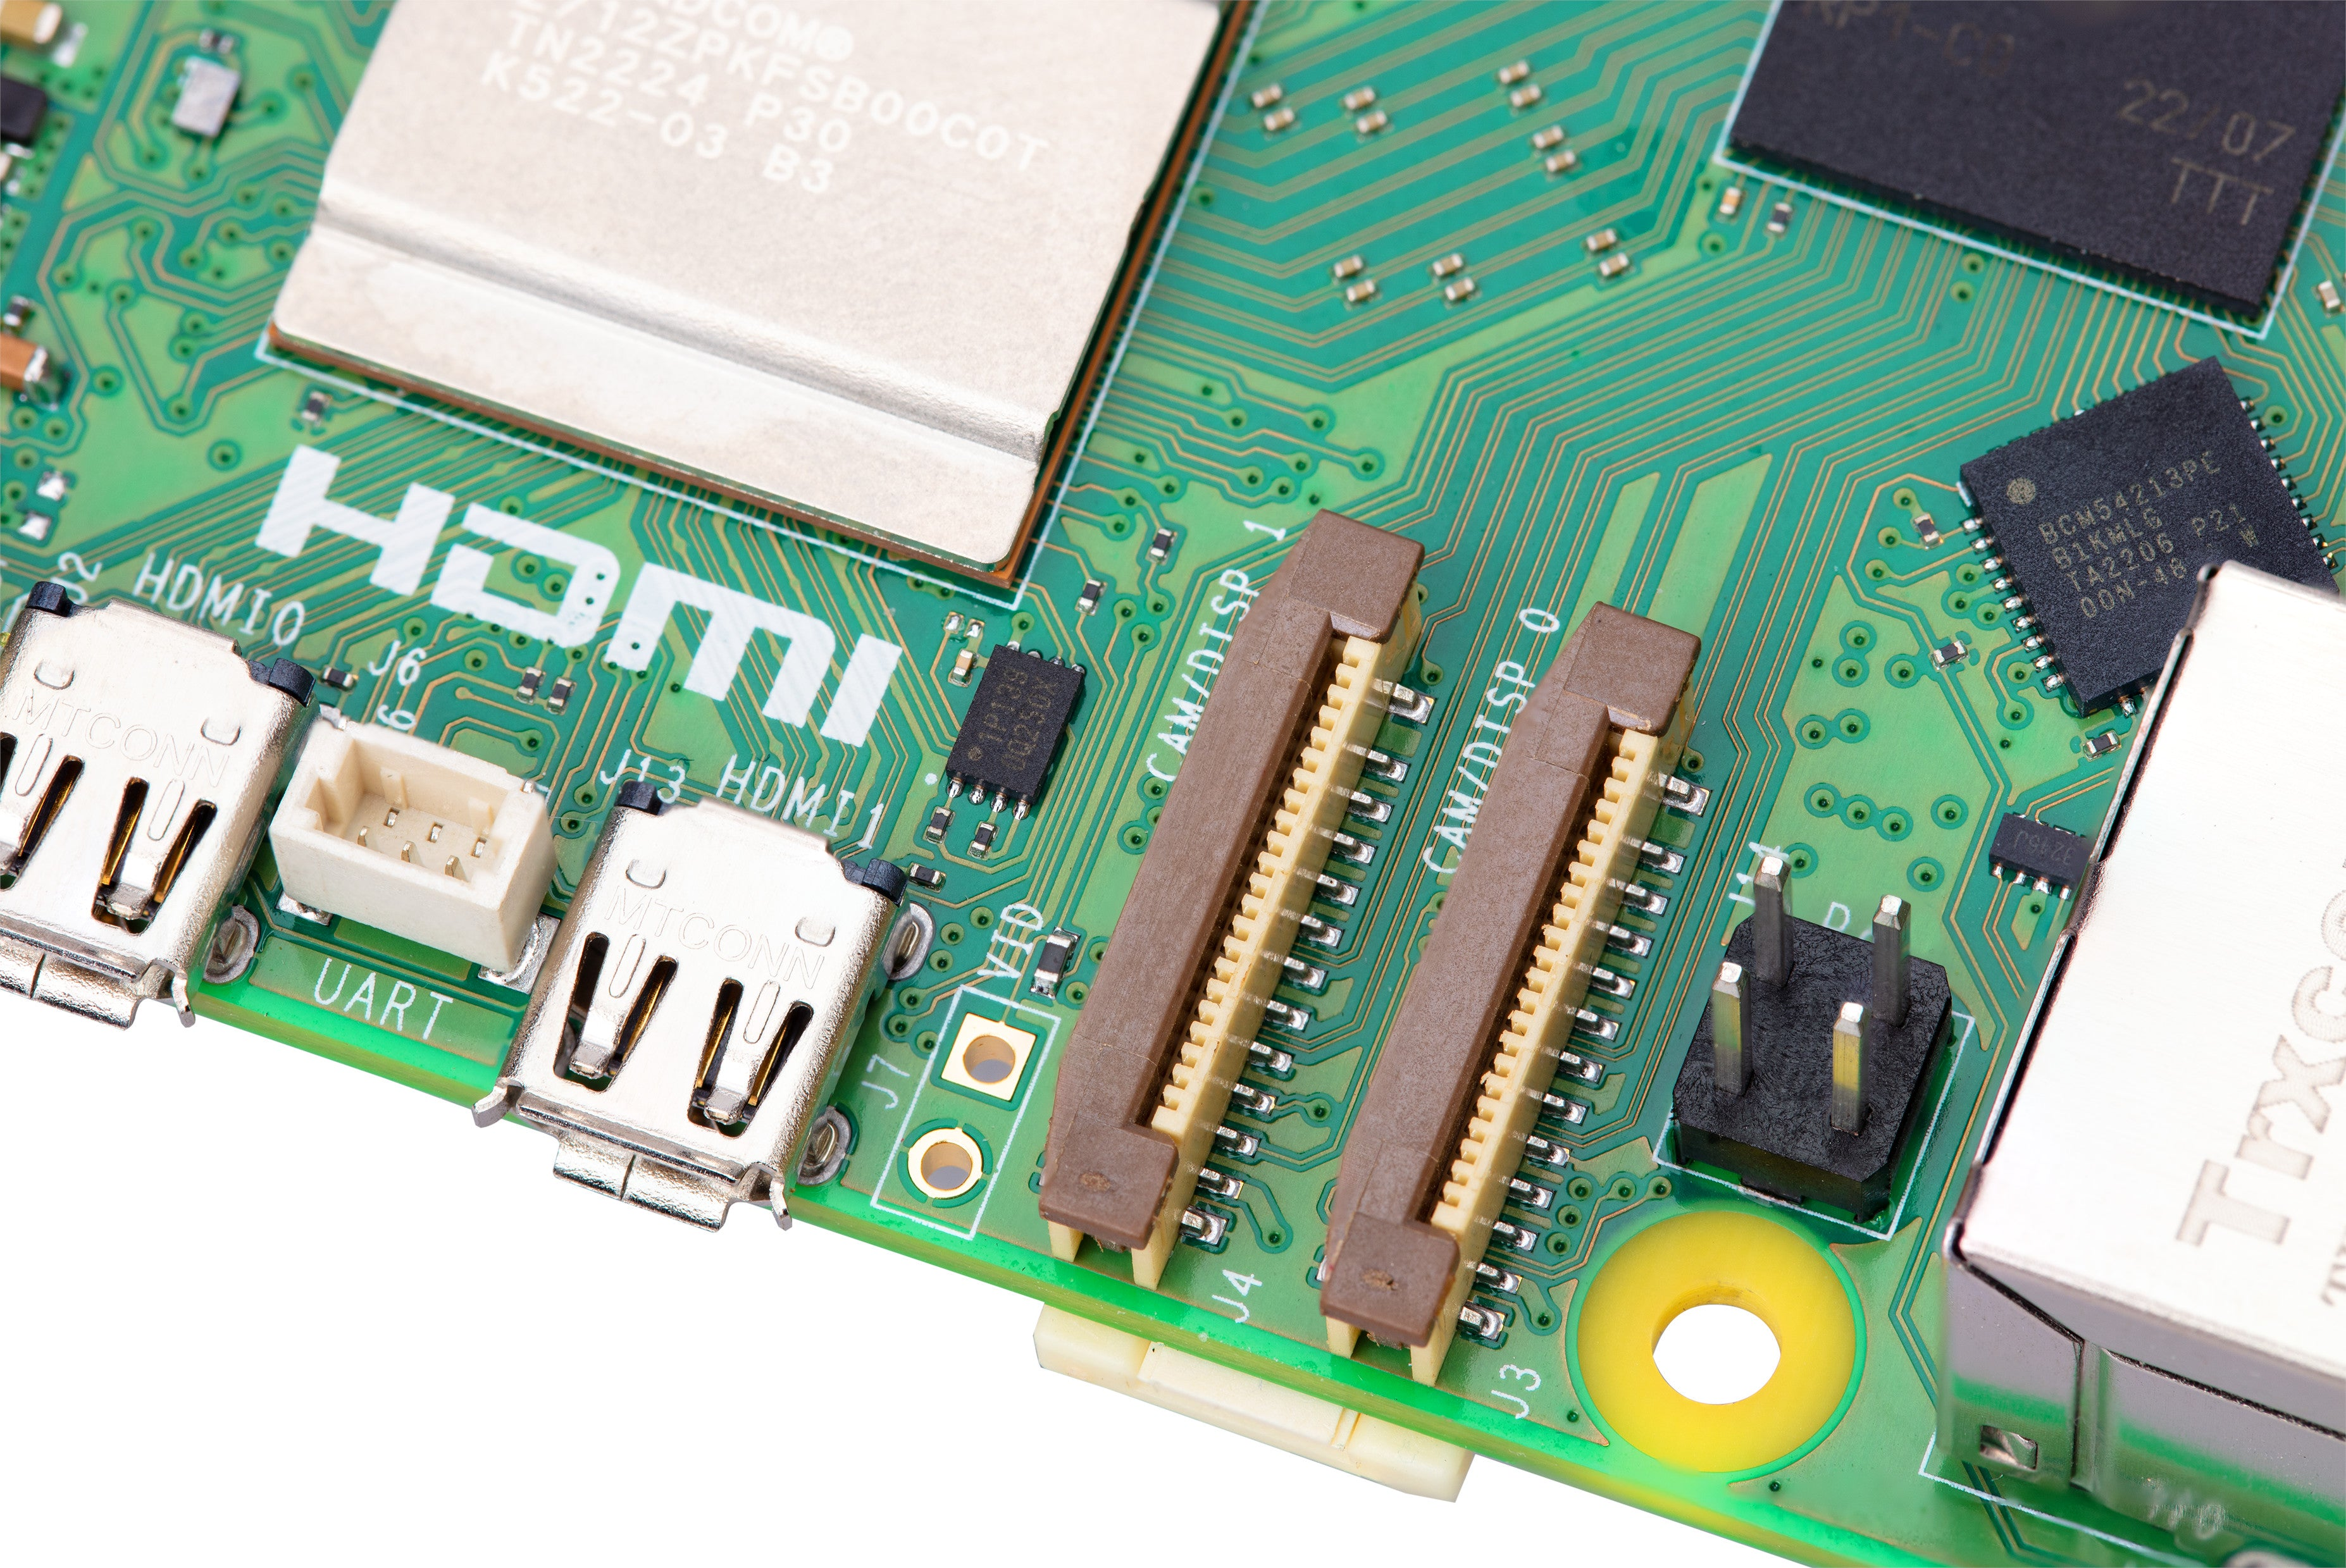
\includegraphics[width=1\textwidth]{images/rpi-5-dsi-csi.jpg}
        \end{figure}

        \column{.4\textwidth} % Right column
        \begin{itemize}
            \item Camera Serial Interface
            \item Modification depuis le Raspberry Pi 5
            \item Sur les anciens modèles, chercher l'indications "CAMERA"
        \end{itemize}

    \end{columns}
\end{frame}

\begin{frame}{Caméra CSI}
    \begin{columns}[c] % 'c' ensures vertical centering for both columns

        \column{.6\textwidth} % Left column
        \begin{figure}
            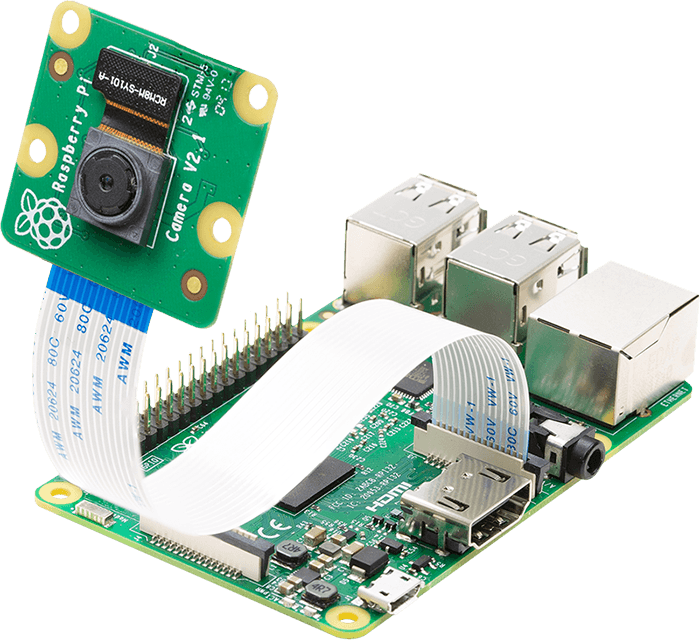
\includegraphics[width=0.6\linewidth]{images/camera-csi.png}
        \end{figure}

        \column{.4\textwidth} % Right column
        \begin{itemize}
            \item 30€-90€
            \item Compacte
            \item Plusieurs modèles et objectifs
            \item Léger pour le processeur
        \end{itemize}

    \end{columns}
\end{frame}


%------------------------------------------------
\section{Prise de photo}
%------------------------------------------------

\begin{frame}{Prise de photo et vidéo}
    \begin{columns}[c] % 'c' ensures vertical centering for both columns

        \column{1\textwidth}
        \begin{itemize}
            \item \texttt{raspistill -o image.jpg} : prend une photo et l'enregistre sous le nom \texttt{image.jpg}
            \item \texttt{raspivid -t 5000 -o video.h264} : prend une vidéo de 5000 milisecondes et l'enregistre sous le nom \texttt{video.h264}
        \end{itemize}

    \end{columns}
\end{frame}

\begin{frame}{Prise de photo et vidéo (avancé)}
    \begin{columns}[c] % 'c' ensures vertical centering for both columns

        \column{1\textwidth}
        \begin{itemize}
            \item \texttt{raspistill}
            \begin{itemize}
                \item \texttt{-t 5000} : minuteur de 5 secondes
                \item \texttt{-rot 180} : rotation de 180 degrés
                \item \texttt{-o image.jpg} : nom du fichier de sortie
                \item \texttt{-awb greyworld} : à utiliser si l'image est rose
            \end{itemize}
            \item \texttt{raspivid}
            \begin{itemize}
                \item \texttt{-t 3000} : temps de 3 secondes
                \item \texttt{-rot 90} : rotation de 90 degrés
                \item \texttt{-o video.h264} : nom du fichier de sortie
                \item \texttt{-awb greyworld} : à utiliser si l'image est rose
            \end{itemize}
            \item \texttt{man raspistill} et \texttt{man raspivid} pour la liste d'options
        \end{itemize}

    \end{columns}
\end{frame}


%------------------------------------------------
\section{Port DSI}
%------------------------------------------------

\begin{frame}{Port DSI}
    \begin{columns}[c] % 'c' ensures vertical centering for both columns

        \column{.6\textwidth} % Left column
        \begin{figure}
            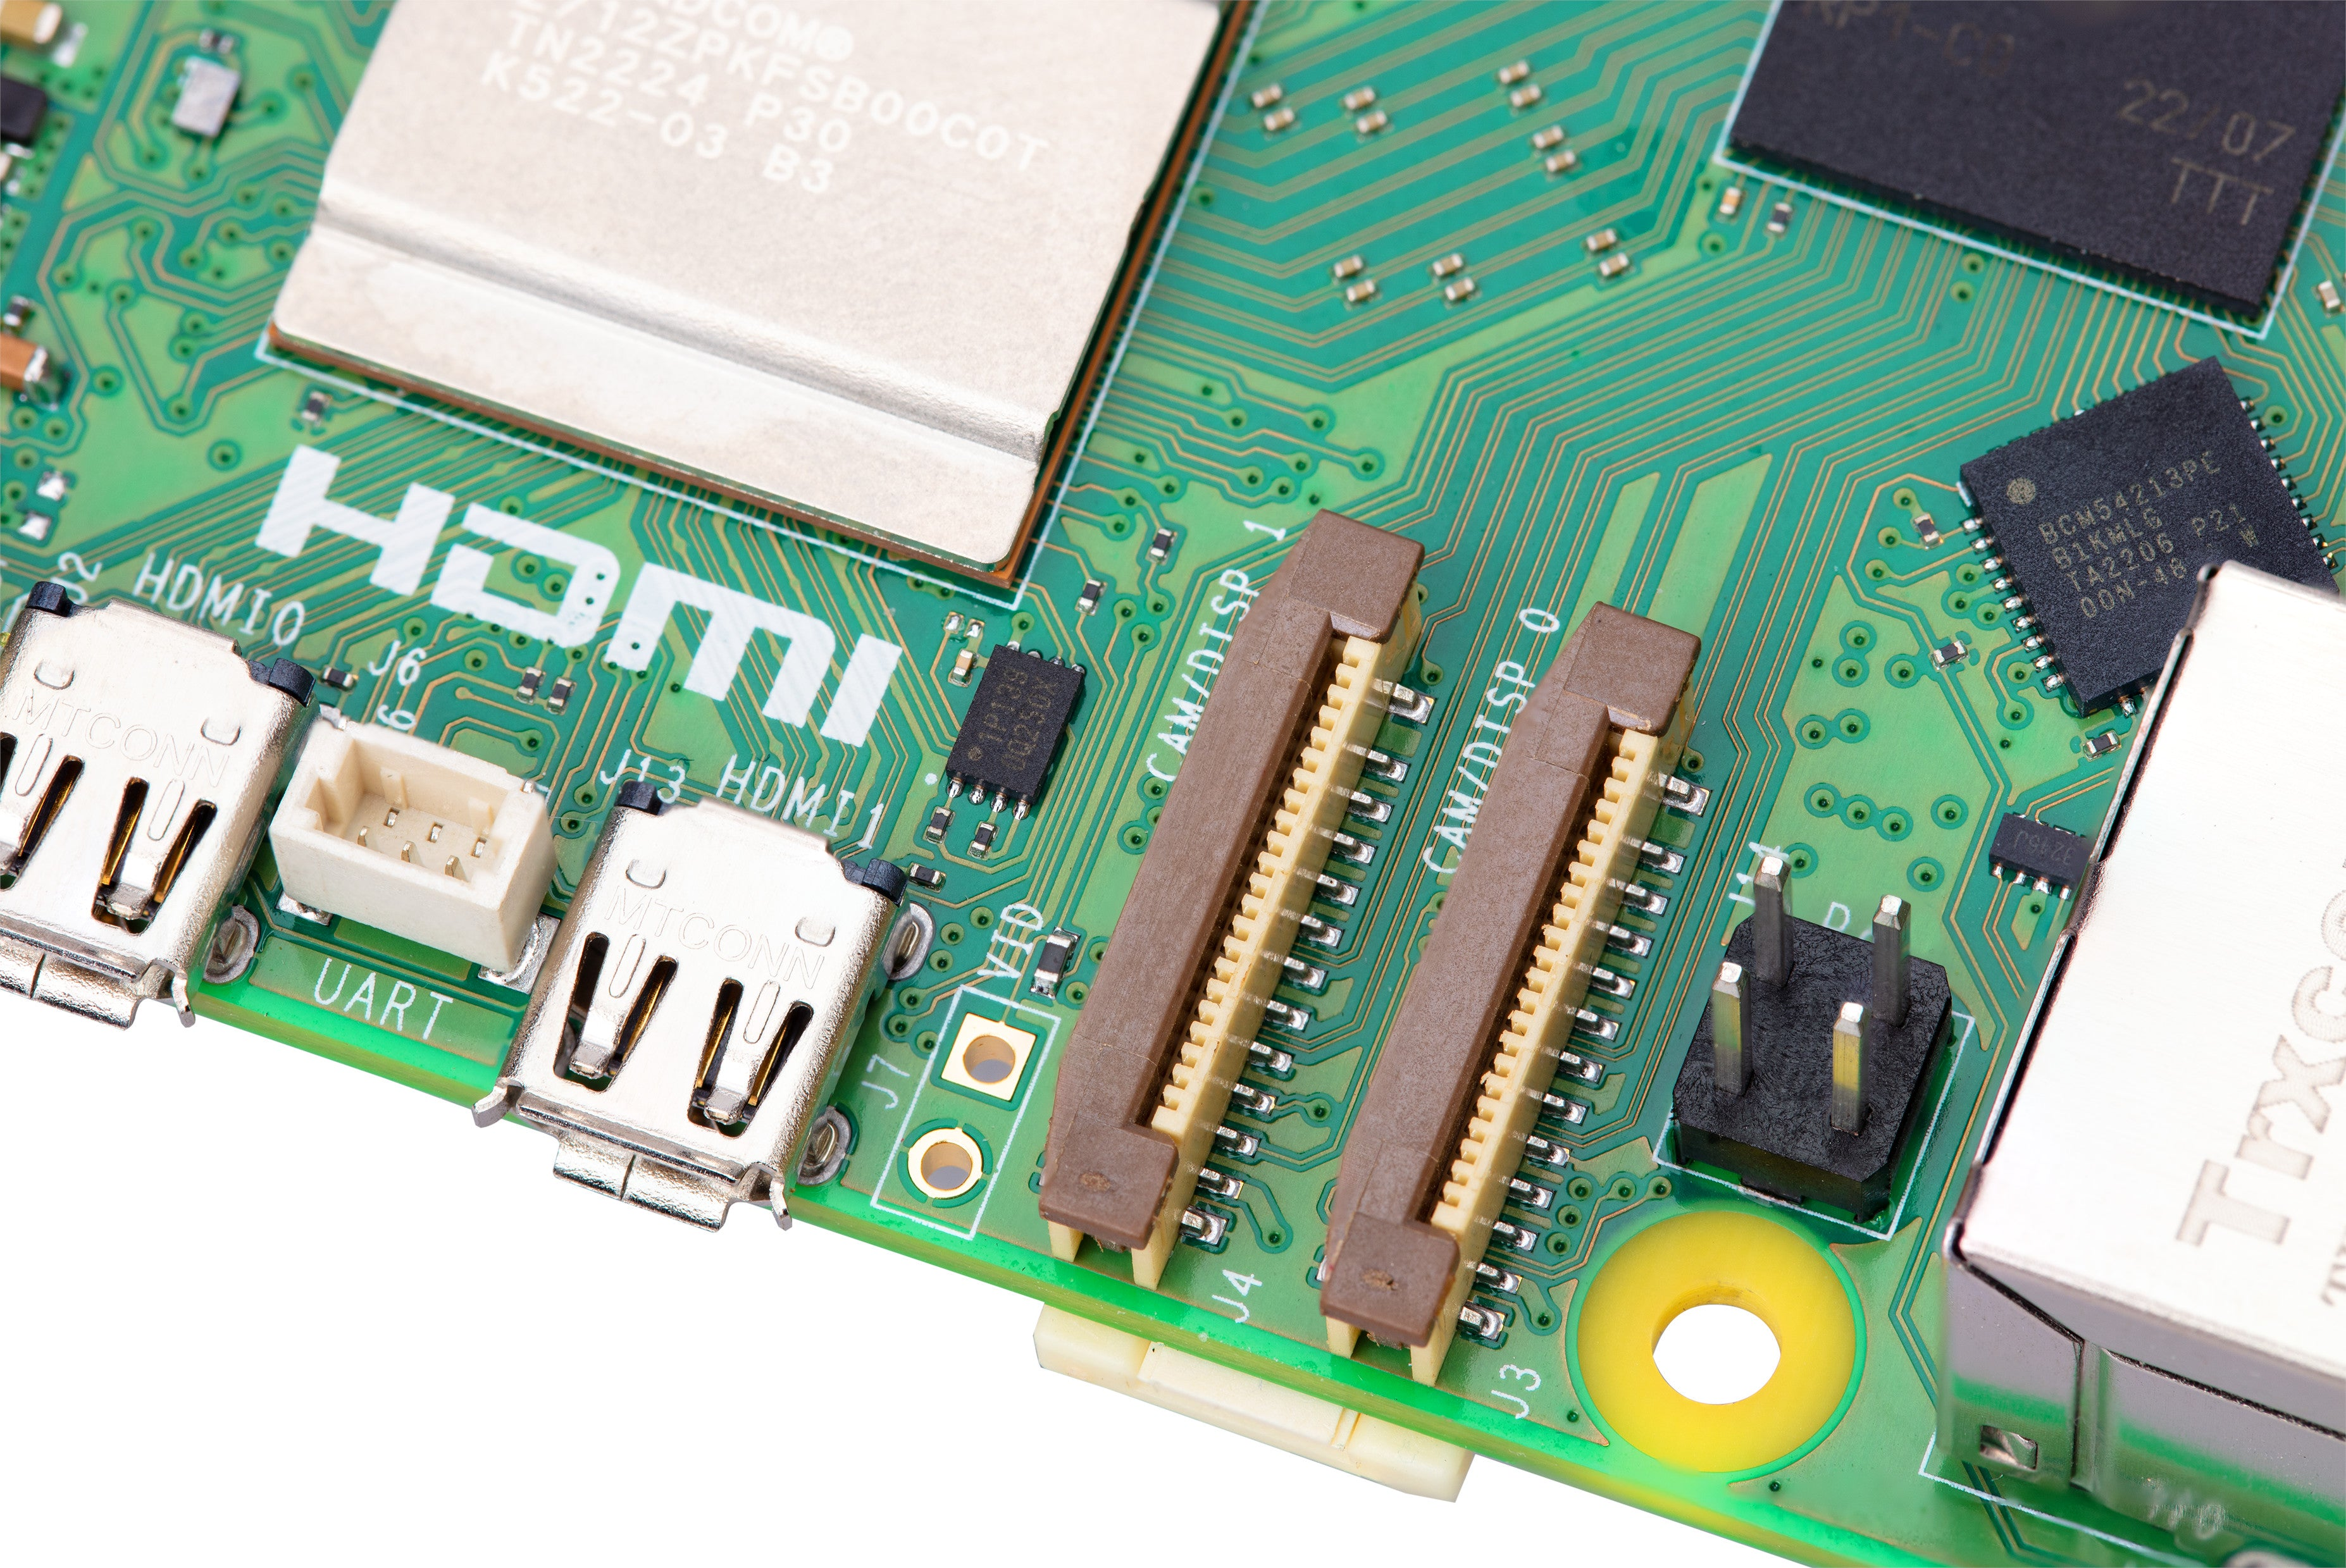
\includegraphics[width=1\textwidth]{images/rpi-5-dsi-csi.jpg}
        \end{figure}

        \column{.4\textwidth} % Right column
        \begin{itemize}
            \item Display Serial Interface
            \item Modification depuis le Raspberry Pi 5
            \item Sur les anciens modèles, chercher l'indications "DISPLAY"
        \end{itemize}

    \end{columns}
\end{frame}

\begin{frame}{Écran DSI}
    \begin{columns}[c] % 'c' ensures vertical centering for both columns

        \column{.6\textwidth} % Left column
        \begin{figure}
            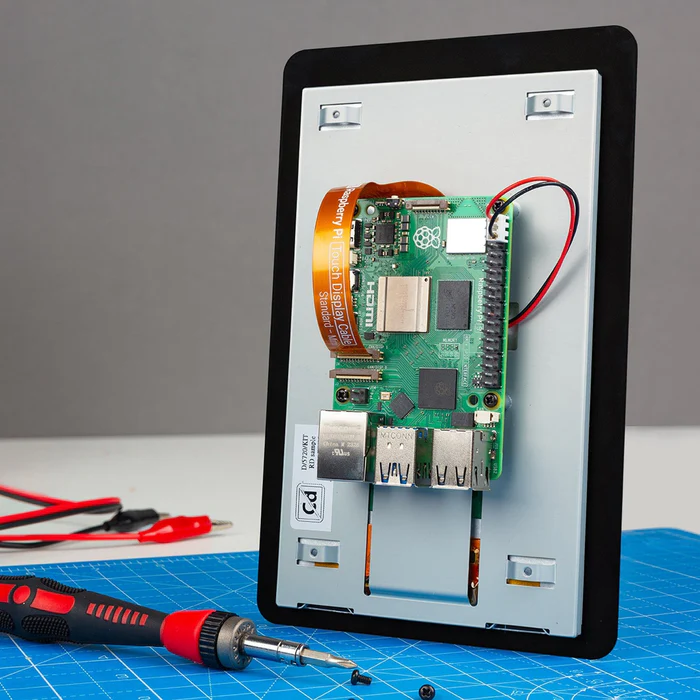
\includegraphics[width=0.8\textwidth]{images/display-dsi.png}
        \end{figure}

        \column{.4\textwidth} % Right column
        \begin{itemize}
            \item 80€
            \item Support des fonctions tactiles
            \item Fixation prévue pour le Raspberry Pi
            \item Faible consommation énergétique
        \end{itemize}

    \end{columns}
\end{frame}


%------------------------------------------------
\section{Photomaton}
%------------------------------------------------
%------------------------------------------------
\section{Vidéosurveillance}
%------------------------------------------------

\end{document}
